
\documentclass[11pt,a4paper]{article}
\usepackage{graphicx}
\usepackage{float}
\usepackage{titlesec}
\usepackage{fancyhdr}
\pagestyle{fancy}
\setcounter{secnumdepth}{4}
\setcounter{tocdepth}{4}
\fancyfoot[C]{\thepage}
\fancyfoot[L,R]{}
\fancyhead[C]{}
\fancyhead[L]{MChessLink UCI Engine}
\fancyhead[R]{Version 1.2.0}
\title{Millennium ChessLink als UCI Schachprogramm}
\author{Lars Nowak}
\date{26.07.2020} 

\begin{document}
\maketitle

\begin{abstract}
Die Idee, die sich hinter dieser Software verbirgt ist, mit dem ChessGenius Exclusive oder dem The King Performance über das Millennium ChessLink-Gerät mit allen Schachprogramm-Oberflächen (in Folge nur kurz GUI
für Graphical User Interface genannt) zu spielen, welche UCI Schachprogramme unterstützen.
Das Millennium ChessLink UCI Schachprogramm (kurz MChessLink) verhält sich gegenüber der GUI wie ein UCI Schachprogramm. D.h. es nimmt die UCI Befehle von der GUI entgegen, sendet die Züge zum Brett und den Antwortzug wieder zurück zur GUI.\\

Ich bin Diplom Informatiker, schreibe die Software in meiner Freizeit und sie ist kostenlos. Ich bin
kein Mitarbeiter der Firma Millennium 2000 GmbH. Millennium ist nicht dafür verantwortlich,
wenn etwas nicht funktioniert. Andererseits kann ich nicht garantieren, dass immer alles funktioniert,
aber ich versuche Fehler so schnell wie möglich zu korrigieren.

\end{abstract}

\newpage
\tableofcontents
\newpage

\section{Vorweg etwas technisches}

\subsection{Unterschiede in den ZIP-Dateien}
Das Programm wird in zwei ZIP-Dateien zur Verfügung gestellt:
\begin{itemize}
\item MChessLinkUci.zip\\
Das Programm basiert auf dem .NET Framework 4.7.1
\item MChessLinkUciCore.zip\\
Das Programm basiert auf .NET Core 3.1.0
\end{itemize}
Sie benötigen nur \textbf{eine} der beiden Dateien. Beide darin enthaltende Programme besitzen die gleiche Funktionalität. Diese beiden Versionen gibt es aus technischen Gründen, die mit der Kommunikation zur GUI zusammenhängen. Wenn sie den HIARCS Chess Explorer (HCE) als GUI einsetzen, müssen sie die
Dateien aus der ZIP-Datei MChessLinkUciCore.zip benutzen.
Sollte sich das .NET Core 3.1.0 noch nicht auf ihrem PC befinden, können sie die notwendigen
Dateien hier herunterladen:
\\ https://dotnet.microsoft.com/download/dotnet-core/3.1

\subsection{Einschränkungen}

Es gibt einige Einschränkungen in der Funktionalität. Sie ergeben sich teilweise auch durch das UCI Protokoll.

\begin{enumerate}
	\item Einige GUIs lassen sich so konfigurieren, dass die ersten Züge aus einem Eröffnungsbuch heraus gespielt werden und die Schachprogramme über die Züge erst dann informiert werden, wenn im Buch keine Züge mehr gefunden werden. In diesem Fall muss die GUI so konfiguriert werden, dass zumindest für das MChessLink-Programm keine Züge aus dem Buch vorgegeben werden.
	\item Um gegen ein anderes, echtes UCI Schachprogramm zu spielen, muss die GUI ein Schachturnier starten, wobei das MChessLink-Programm eines der Teilnehmer ist. Arena bietet eine Aussnahme, die später erklärt wird.
	\item Die Kommunikation mit dem Schachbrett erfolgt über einen Gerätetreiber, welcher den USB-Anschluss auf einen (virtuellen) Seriellen-Anschluss umleitet.  Den Hersteller des Gerätetreibers für das ChessLink-Gerät finden sie unter: \\ https://www.ftdichip.com/Drivers/VCP.htm
	\\Folgen sie der Anleitung von Millennium für die Installation des Millennium ChessLink.
\end{enumerate}

\pagebreak

\section{Kurzanleitng}
\begin{itemize}
	\item Entpacken sie \textbf{eine} der beiden ZIP-Dateien in einen eigenen Ordner. Die ZIP-Dateien beinhalten folgende Dateien.
    \begin{itemize}
		\item MChessLinkUci.zip
      	\begin{enumerate}
  		 	\item MChessLinkUci.exe
			\item MChessLinkChessBoard.dll
			\item MChessLinkEBoardWrapper.dll
			\item CommonUciWrapper.dll
			\item BearChessBase.dll
		\end{enumerate}
	    \item MChessLinkCore.zip
		   \begin{enumerate}
			   	\item MChessLinkUciCore.exe
				\item MChessLinkCore.dll
				\item MChessLinkCore.deps.json
				\item MChessLinkCore.runtimeconfig.json
				\item System.IO.Ports.dll
    			\item MChessLinkChessBoard.dll
                \item MChessLinkEBoardWrapper.dll
                \item CommonUciWrapper.dll
                \item BearChessBase.dll
				\item runtimes
		   \end{enumerate}
    \end{itemize}
	\item Verbinden sie das Millennium ChessLink-Gerät mit ihrem Computer und mit dem Millennium Schachbrett.
	\item Bauen sie die Schachfiguren in ihrer Grundstellung auf. Die weißen Steine müssen sich auf der Grundreihe befinden, auf der die Millennium-Plakette angebracht ist.
	\item Schalten sie das ChessLink-Gerät ein.
	\item Für King Performance: Aktivieren sie den ChessLink-Modus (\textbf{CLink}) und drücken \textbf{New} für eine neue Partie.
	\item Starten sie die GUI (z.B. Fritz, HIARCS Chess Explorer oder Arena) und installieren das MChessLink-Programm als ein UCI-Schachprogramm.
	\item Beginnen sie ein Schachturnier und wählen das MChessLink-Programm als einen der Teilnehmer aus.
\end{itemize}


\section{Verzeichnisse}
Nach dem ersten Start erzeugt das Programm verschiedene Verzeichnisse:
\begin{enumerate}
	\item \begin{verbatim}
C:\Users\YOURUSERS\AppData\Local\MChessLinkUci
	\end{verbatim} 
	\item\begin{verbatim}
	C:\Users\YOURUSERS\AppData\Local\MChessLinkUci\log
	\end{verbatim} 
	\item \begin{verbatim}
	C:\Users\YOURUSERS\AppData\Local\MChessLinkUci\engines
	\end{verbatim} 	
		\item \begin{verbatim}
	C:\Users\YOURUSERS\AppData\Local\MChessLinkUci\books
	\end{verbatim} 	
\end{enumerate}
\begin{quote}
YOURUSERS ist der Platzhalter für ihr Windows Benutzername.
\end{quote}

Das erste Verzeichnis enthält eine Konfigurationsdatei. In dem zweiten Verzeichnis werden Protokoll-Dateien abgelegt.\\Wenn sie UCI-Schachprogramme in das dritte Verzeichnis kopieren, können sie später in dem Konfigurationsdialog ausgewählt werden.\\Kopieren sie Polyglot- oder Arena-Eröffnungsbücher in das Books-Unterverzeichnis.

\section{Konfiguration}

\begin{figure}[H]
	\centering
	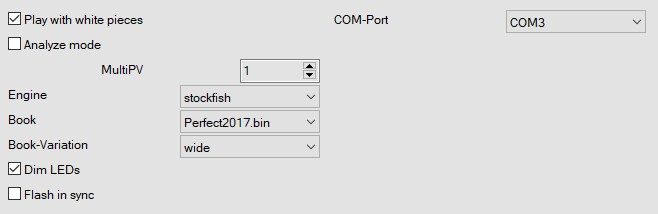
\includegraphics[scale=0.7]{configuration.jpg}
	\caption{Konfiguration}
	\label{fig:configration}
\end{figure}
\begin{itemize}

	\item \textbf{Play with white pieces} Wenn die Auswahl nicht gesetzt ist, spielen sie mit den schwarzen Figuren. D.h. das Brett ist gedreht.

	\item \textbf{MultiPV} Setzt die Anzahl der parallelen Analysen eines Schachprogramms. Die Option ist nur verfügbar, wenn sie weitere UCI-Schachprogramme in das Engines-Unterverzeichnis kopiert haben. Bei einem Schachturnier wird die Angabe ignoriert. Mit Ausnahme von Arena wird diese Option auch gar nicht angezeigt.
	
	\item \textbf{Engine} Wählen sie ein UCI-Schachprogramm aus, welches sich im Engine-Unterverzeichnis befindet.

    \item \textbf{Analyze mode} Benutzen sie das ausgewählte Schachprogramm zur Analyse ihrer Züge. Die Option ist nur verfügbar, wenn sie weitere UCI-Schachprogramme in das Engines-Unterverzeichnis kopiert haben.
    
    \item \textbf{Book} Auswahl eines Eröffnungsbuches. Die Option ist nur verfügbar, wenn sie eigene Eröffnungsbücher in das Books-Unterverzeichnis kopiert haben.
   \item \textbf{Book-Variation} Bestimmt, wie das Eröffnungsbuch eingesetzt wird.
   \begin{itemize}
   	  \item \textbf{best move} Es wird immer der beste Zug ausgewählt.
   	  \item \textbf{flexible} Bei der Auswahl wird die Gewichtung bzw. Priorisierung berücksichtig.   	  \item \textbf{wide} Ein Zug wird zufällig ausgewählt. 
   \end{itemize}
    \item \textbf{COM-port} Wenn das automatische Erkennen des COM-Anschlusses nicht funktioniert, müssen sie hier den richtigen COM-Anschluss auswählen. In der Regel müssen sie das tun, wenn mehrere COM-Anschlüsse zur Verfügung stehen.
    \item \textbf{Dim LEDs} In der Voreinstellung sind die LEDs auf dem Schachbrett sehr hell. Über diese Option können sie ein wenig abgedunkelt werden.
    \item \textbf{Flash in sync} Bestimmen sie, ob die LEDs der Felder für den Schachzug synchron oder abwechselnd blinken.

\end{itemize}

\subsection{Die Intention hinter 'Analyze mode', 'UCI engine' und 'Opening book'}
In den meisten Fällen müssen sie in der Konfiguration kein UCI-Schachprogramm bzw. Eröffnungsbuch auswählen oder es macht keinen Sinn es zu tun. Insbesondere dann nicht, wenn sie ein Turnier spielen, da der Gegener von der GUI bestimmt wird.
\\Die Idee, eine UCI-Schachprogramm innerhalb des MChessLink-Programm zu definieren, ist das Schachprogramm für eine Analyse einzusetzen, während sie ihre Züge auf dem Schachbett machen. Dafür aktivieren sie in der Konfiguration den ``Analyze mode``. Nicht zu Verwechseln mit einer Spielanalyse, welche einige GUIs anbieten.\\
Einige GUIs erlauben einem Schachprogramm gegen sich selbst zu spielen, ohne dafür ein ganzes Turnier zu eröffnen. Z.B. erreichen sie das mit Arena, in dem sie einfach den ``Demo`` Knopf anklicken. So können sie das MChessLink-Programm nutzen um gegen einen anderen, menschlichen Gegner zu spielen und sich gleichzeitig die Analyse der Züge anzuschauen oder einfach nur die Züge zu protokollieren.

\newpage
\section{Anwendungsbeispiele}
Die folgenden Kapitel beschreiben einige Szenarien und wie sie in verschiedenen GUIs umgesetzt werden können. Bitte haben sie dafür Verständnis, dass die Szenarien nur für einige GUIs und mit englischen Screenshots beschrieben werden und es möglicherweise mit anderen GUIs nicht reibungslos funktioniert.
\subsection{Gegen ein anderes UCI-Schachprogramm spielen}
\subsubsection{Fritz}
\paragraph{Schachturnier}
\begin{enumerate}
	\item Starten sie ein neues Schachturnier.
	\begin{figure}[H]
		\centering
		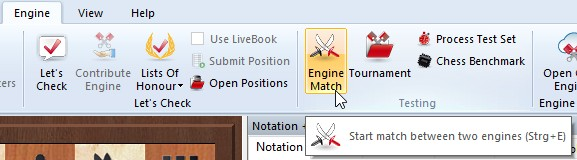
\includegraphics[scale=0.6]{fritz_enginematch.jpg}
		\caption{Fritz Engine Match}
		\label{fig:FritzEngineMatch}
	\end{figure}
	\item Wählen sie für Weiss das MChessLink-Programm.
		\begin{figure}[H]
		\centering
		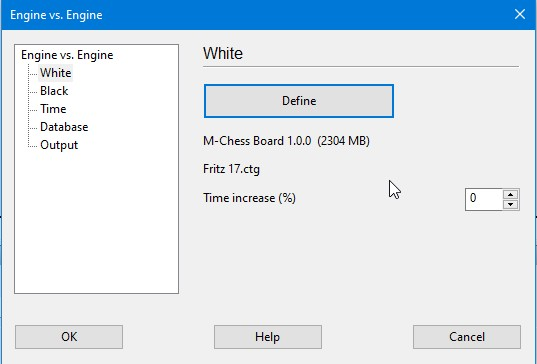
\includegraphics[scale=0.7]{fritz_enginewhite.jpg}
		\caption{Define Engine for White}
		\label{fig:FritzEngineWhite}
	\end{figure}
	\item Öffnen sie den Konfigurationsdialog. Deaktivieren sie ``Analyze mode`` und wählen ``\begin{math}<none>\end{math}`` als Engine.
			\begin{figure}[H]
		\centering
		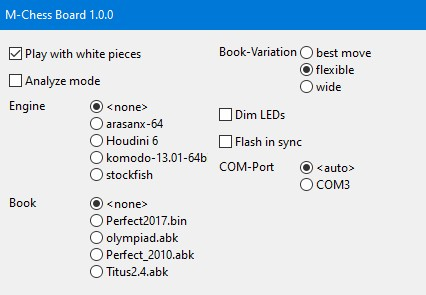
\includegraphics[scale=0.8]{fritz_engine_configure_mchesslink.jpg}
		\caption{Configure MChessLink Engine}
		\label{fig:FritzConfigureCertabo}
	\end{figure}

	\item Stellen sie sicher, dass ``Use book`` nicht aktiviert ist.
		\begin{figure}[H]
		\centering
		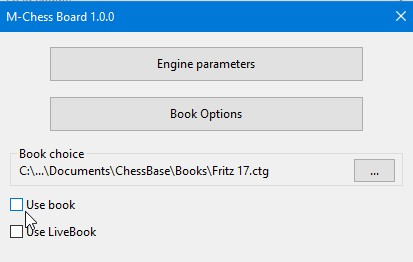
\includegraphics[scale=0.8]{fritz_engineusebook.jpg}
		\caption{Use Book}
		\label{fig:FritzUseBook}
	\end{figure}
	\item Wählen sie für Schwarz ein installiertes Schachprogramm aus.
	\item Setzen sie die Zeitkontrolle und starten das Turnier.	
\end{enumerate}

\subsubsection{Arena}
Arena erlaubt verschiedene Möglichkeiten, gegen ein anderes Schachprogramm zu spielen. Allen gemeinsam ist, dass das MChessLink-Programm nicht das Arena-Eröffnungsbuch benutzen darf. Deaktivieren sie dazu die Option ``Use Arena general main books with this engine``.
\begin{figure}[H]
	\centering
	\includegraphics[scale=0.7]{arena_mainbooks.jpg}
	\caption{MChessLink Arena Book}
	\label{fig:ArenaUseBook}
\end{figure}
\paragraph{Mit einem MChessLink-Programm und einem UCI-Schachprogramm}
\begin{enumerate}
\item Laden sie das  MChessLink-Programm als \mbox{``Engine 1``} und das gegnerische Programm als \mbox{``Engine 2``}.
	\begin{figure}[H]
	\centering
	\includegraphics[scale=0.7]{arena_engine1.jpg}
	\caption{MChessLink-Programm as Engine 1}
	\label{fig:ArenaEngine1}
\end{figure}
\item Konfiguration der Engine 1 (MChessLink-Programm)
\begin{figure}[H]
	\centering
	\includegraphics[scale=0.6]{arena_configureengine1.jpg}
	\caption{Configuration Engine 1}
	\label{fig:ArenaConfigureEngine1}
\end{figure}
\item Öffnen sie den Konfigurationsdialog. Deaktivieren sie ``Analyze mode`` und wählen ``\begin{math}<none>\end{math}`` als Engine.
\begin{figure}[H]
	\centering
	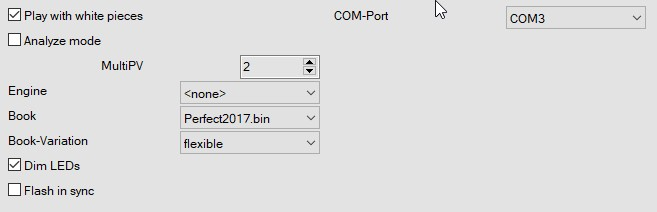
\includegraphics[scale=0.7]{Arena_ConfigureMChessLink.jpg}
	\caption{Configuration MChessLink-Programm}
	\label{fig:ArenaConfigureCertabo}
\end{figure}
\item Klicken sie auf  ``Demo`` um das Spiel zu beginnen.
\begin{figure}[H]
	\centering
	\includegraphics[scale=0.7]{arena_demo.jpg}
	\caption{Start with ``Demo``}
	\label{fig:ArenaDemo}
\end{figure}
\end{enumerate}

\paragraph{Einzeln geladenes MChessLink-Programm}
\subparagraph{} Wenn Sie in das Engine-Unterverzeichnis ein UCI-Schachprogramm kopiert haben, können sie es direkt als Gegner einsetzen.
\begin{enumerate}
	\item Schließen sie ggf. die geladene ``Engine 2``.
	\begin{figure}[H]
		\centering
		\includegraphics[scale=0.7]{arena_closeengine2.jpg}
		\caption{Close Engine 2}
		\label{fig:ArenaCloseEngine2}
	\end{figure}
    \item Öffnen sie den Konfigurationsdialog für das MChessLink-Programm. Deaktivieren sie den ``Analyze mode`` und wählen ein UCI-Schachprogramm aus.
    	\begin{figure}[H]
    	\centering
    	\includegraphics[scale=0.7]{arena_ConfigureMChessLink2.jpg}
    	\caption{Select an UCI Engine}
    	\label{fig:ArenaConfigureCertabo2}
    \end{figure}
    \item Klicken sie auf ``Demo`` um das Spiel zu beginnen.
    \begin{figure}[H]
    	\centering
    	\includegraphics[scale=0.7]{arena_demo.jpg}
    	\caption{Run Demo}
    	\label{fig:ArenaDemo}
    \end{figure}
\end{enumerate}

\paragraph{Schachturnier}
\begin{enumerate}
\item Beginnen sie ein Schachturnier
  \begin{figure}[H]
	\centering
	\includegraphics[scale=0.7]{arena_enginetournament.jpg}
	\caption{Arena Engine Tournament}
	\label{fig:ArenaEngineTournament}
\end{figure}
\item Stellen sie für das MChessLink-Programm sicher, dass der ``Analyze mode`` deaktiviert und ``\begin{math} <none> \end{math}`` als Engine ausgewählt ist.
\end{enumerate}
Sie können das MChessLink-Programm zweimal unter verschiedenen Namen definieren. Somit können sie z.B. ein Turnier gegen sich selbst, mit unerschiedlichen UCI-Schachprogrammen zur Analyse, spielen.

\subsection{Analysieren mit einem UCI-Schachprogramm}
Während sie ihre Schachzüge ausführen, wird ihnen die Analyse des UCI-Schachprogramms angezeigt. Eröffnungsbücher werden ignoriert.
\subsubsection{Fritz}
\paragraph{Engine Turnier}
\begin{enumerate}
	\item Starten sie ein neues Turnier.
	\begin{figure}[H]
		\centering
		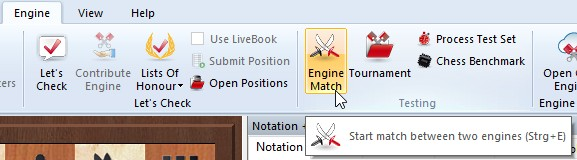
\includegraphics[scale=0.6]{fritz_enginematch.jpg}
		\caption{Fritz Engine Match}
		\label{fig:FritzEngineMatch}
	\end{figure}
	\item Wählen sie für Weiß das MChessLink-Programm.
	\begin{figure}[H]
		\centering
		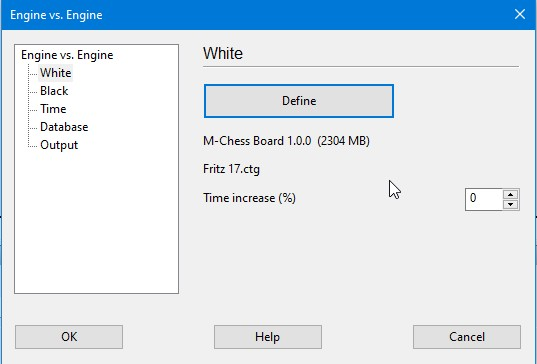
\includegraphics[scale=0.6]{fritz_enginewhite.jpg}
		\caption{Define Engine for White}
		\label{fig:FritzEngineWhite}
	\end{figure}
	\item Öffnen sie für MChessLink den Konfigurationsdialog, aktivieren den ``Analyze mode`` und wählen ein UCI-Schachprogramm aus.
	\begin{figure}[H]
		\centering
		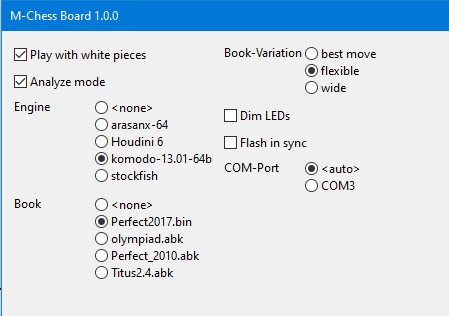
\includegraphics[scale=0.8]{fritz_engine_configure_mchesslink_analyze.jpg}
		\caption{Configure MChessLink Engine}
		\label{fig:FritzConfigureCertabo}
	\end{figure}
	
	\item Überpüfen sie, dass ``Use book`` nicht ausgewählt ist.
	\begin{figure}[H]
		\centering
		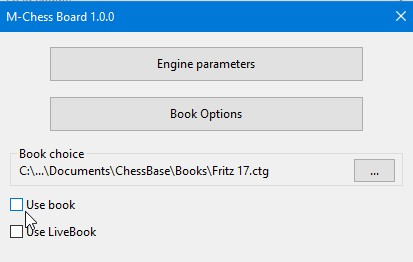
\includegraphics[scale=0.6]{fritz_engineusebook.jpg}
		\caption{Use Book}
		\label{fig:FritzUseBook}
	\end{figure}
	\item Wählen sie für Schwarz ein in Fritz installiertes Schachprogramm aus.
	\item Setzen sie die Zeitkontrolle und starten das Turnier.	
\end{enumerate}
\subsubsection{Arena}
Sie können in Arena, genauso wie zuvor für Fritz beschrieben, ein Schachturnier starten. Arena bietet aber über den Demo-Modus eine weitere Lösung an. Installieren sie unter Arena das MChessLink-Programm zweimal mit unterschiedlichen Namen. So können sie jeweils eine eigene Konfiguration abspeichern. Lassen sie so zwei MChessLink-Programme mit unterschiedlichen UCI-Programmen gegeneinander spielen und nutzen deren eigene Analyse. Arena bietet, etwas abseits des UCI-Protokolls hier die Möglichkeit, den MultiPV-Parameter zu setzen. So kann die Analyse für mehrere Zugvarianten angezeigt werden.

\subsection{Start von einer beliebigen Position}
Sie können von einer beliebigen Schachposition starten, die sie in der GUI aufgebaut haben. Am besten, sie platzieren die Figuren zuerst auf dem Millennium Schachbrett und öffnen dann die Positionseingabe in ihrer GUI.
\subsubsection{Arena}
\begin{enumerate}
  \item Öffnen sie den Dialog zum Aufbau einer Position.
  \item Schließen sie den Dialog und Klicken auf ``Demo`´. Die LEDs auf dem Schachbrett blinken für alle nicht korrekt aufgestellten oder fehlenden Figuren.
\end{enumerate}

\section{Wichtig zu Wissen}
\subsection{Protokoll-Dateien}
Das MChessLink-Programm schreibt mindestens zwei Protokoll-Dateien in das Log-Unterverzeichnis:
\begin{enumerate}
  \item mchesslinkUci\_1.log
  \item mchesslink\_1.log
\end{enumerate}
Startet die GUI zwei MChessLink-Programme gleichzeitig, z.B. wenn sie ein Turnier gegen zwei MChessLink-Programme spielen, werden weitere Protokoll-Dateien mit den Namen mchesslinkUCi\_2.log und mchesslink\_2.log angelegt.


\subsection{COM port}
Das Programm ermittelt alle verfügbaren COM-Anschlüsse und benutzt den ersten, freien Anschluss. Stellt ihr Computer mehrere Anschlüsse zur Verfügung, kann es zu einer Fehlkonfiguration kommen. Wenn Sie den COM-Port wechseln, müssen sie ggf. das Programm neu starten.

\subsection{Opening books}
Das Programm unterstützt Polyglot- und Arena-Eröffnungsbücher. Die interne Struktur beider Eröffnungsbücher ist sehr unterschiedlich. Vereinfacht ausgedrückt ist Polyglot stellungsorientiert und Arena-Bücher zugorientiert. Sie können daher ein Polyglot-Buch benutzen, wenn sie von einer beliebigen Position die Partie beginnen. Bei einem Arena-Buch müssen sie von der Grundstellung aus starten.

\section{Fehlerbehebung}


\subsection{Die Schachzüge werden nicht korrekt angezeigt}
\begin{itemize}
	\item Überprüfen sie, ob der richtige COM-Port konfiguriert ist.
	\item Vergewissern sie sich, dass die Figuren korrekt aufgestellt sind. Solange die Figuren nicht auf dem erwarteten Feld stehen, werden keine Züge akzeptiert. Bei Feldern mit falschen oder fehlenden Figuren blinken die LEDs.
	\item Versuchen sie alternativ die Dateien aus der Datei MChessLinkUciCore.zip.
	\item Das UCI-Protokoll ist zwar gut dokumentiert, aber nicht jede GUI sendet die Kommandos in der gleichen Art und Weise. Ich teste das Programm unter den verbreitesten GUIs, aber es kann immer wieder zu Änderungen kommen.
\end{itemize}

\subsection{Das Programm zieht selbständig seine Züge}
\begin{itemize}
\item Wenn sie ein Turnier spielen, öffnen sie den Konfigurationsdialog und aktivieren den ``Analyze mode`` oder wählen als UCI-Engine ``\begin{math}<none>\end{math}`` aus.
\item Überprüfen sie, dass die GUI die Züge nicht aus einem Eröffnungsbuch wählt.
\end{itemize}

\section{Bekannte Probleme}
\begin{itemize}
	\item Aktuell müssen die weißen Figuren auf der Gundreihe aufgestellt werden, wo sich die Millennium-Plakette befindet. 
    \item Beim zu schnellen Ziehen der Figuren kann es passieren, dass der Zug nicht richtig erkannt wird. In diesem Fall den Zug wiederholen.
	\item Wenn ein Zug nicht (mehr) im Eröffnungsbuch gefunden wird, werden auch die Folgezüge nicht mehr in dem Buch gesucht.
\end{itemize}

\section{Next Steps}
\begin{itemize}
	\item Verbesserung de COM-Port Erkennung.
	\item Verbesserung der Zugerkennung.
	\item Fehlerbeseitigung.
\end{itemize}

\pagebreak

\section{Changelog}
\subsection{26.07.2020 =\textgreater Dokumentation überarbeitet}
\subsection{Version 1.1.2 =\textgreater 1.2.0}
\begin{itemize}
	\item Starke Verbesserung bei der Zugerkennung.
\end{itemize}
\subsection{Version 1.1.1 =\textgreater 1.1.2}
\begin{itemize}
	\item Fehlerbehebung bei der langen Rochade. Der Turm wurde intern auf ein falsche Feld plaziert.
\end{itemize}
\subsection{Version 1.1.0 =\textgreater 1.1.1}
\begin{itemize}
	\item Fehlerbehebung für die HCE-GUI durch den Einsatz von .Net Core
\end{itemize}
\subsection{Version 1.0.1 =\textgreater 1.1.0}
\begin{itemize}
	\item Fehlerbehebung der LED-Anzeige für Feld D5 .
    \item Bessere Zugerkennung wenn die Figuren langsam über das Brett gezogen werden, sogenanntes ``Schleifen``.
    \item Optimierungen innheralb des Programmcodes.
\end{itemize}
\subsection{Version 1.0.0 =\textgreater 1.0.1}
\begin{itemize}
	\item Fehlerkorrektur bei der COM-Port-Konfguration.
\end{itemize}


\end{document}